\chapter{Experiments and results}
\label{chap:Experimentos e resultados}
\lettrine{I}{n} this chapter, the experiments carried out and the results obtained will be presented.
To this end, we will begin by presenting an overview of the experimentation process,
followed by the experiments themselves, to finally analyze the results obtained as a whole and the conclusions that can be drawn from them.

\section{Overview}
\label{sec:Vista Xeral}

The objective of this work is to determine if implicit networks are suitable for the retinal registration task. The main comparison focuses on the activation function used (SIREN or ReLU), on the FIRE and RFMID datasets.

The initial evaluation on the FIRE dataset, as can be seen in figures \ref{fig:FIRE_relu} and \ref{fig:FIRE_SIREN}, showed limited performance. Category P proved impossible to register, probably due to the low degree of overlap between images (<75%), while categories S and A barely achieved success rates of 20%.

With the aim of improving this performance and understanding the key factors that influence registration, a series of systematic experiments was designed. This section provides an overview of each of these experiments, advancing their motivation and main findings, which will be detailed in the rest of the chapter.

\begin{itemize}
\item \textbf{Loss function:} The motivation was to find the most robust similarity metric for retinal images, which present great variability in contrast and illumination. The main finding was that the optimal choice depends on the nature of the images: for real images with variability (FIRE), functions based on structural features like NCC offered the best results; for synthetic images without such variability (RFMID), pixel-based functions like L1 were superior.

\item \textbf{Image resolution:} It was investigated whether the high resolution of retinal images (up to 2160x2160) provided a significant benefit compared to the computational cost. The conclusion was that, although very low resolutions were insufficient, no notable improvement was observed above 1250x1250 pixels, establishing this value as a good balance between detail and efficiency.

\item \textbf{Regularization:} This experiment was crucial to avoid unrealistic deformations, a particular risk in SIREN models due to their bias towards high frequencies. It was confirmed that some degree of regularization is indispensable, but the optimal amount of regularization is not universal, rather it depends on the complexity of the transformation.

\item \textbf{Batch size:} Qualitative analysis suggested this was a high-impact parameter. The experiments confirmed it is one of the most critical factors for registration success. A large batch size (e.g., 10000 or more) is fundamental for obtaining good results.

\item \textbf{Sampling strategies:} The initial hypothesis was that prioritizing regions with more information (blood vessels, optic disc) through "intelligent" sampling strategies would improve performance. The results showed that none of the proposed strategies (uniform, weighted) offered a significant advantage over traditional random sampling.

\item \textbf{Initialization:} Given the non-convex nature of the optimization problem, it was explored whether a careful selection of initial weights could improve convergence. An "initialization lottery" was implemented that chooses the best of several initial runs. A marginal but consistent improvement was observed, indicating that initialization has some impact, although it is not a transformative factor.

\item \textbf{Dynamic batch size adjustment:} The strategy of starting with a small batch size to learn the global transformation and then increasing it to refine local details was tested. The result was conclusive and contrary to the hypothesis: this strategy proved to be detrimental, worsening performance. A large and constant batch size from the start proved to be more effective.

\end{itemize}

Unless otherwise specified, for the experiments a learning rate of 0.0001, batch size of 10000 points and 1500 epochs will be used. These values were determined from those originally used by IDIR and from qualitative analysis of results obtained in preliminary experiments. The set of these experiments allows building a detailed understanding of the strengths and weaknesses of implicit networks in this task.

\begin{figure}[tbp]
    \centering
    \begin{subfigure}[b]{0.5\textwidth}
        \centering
        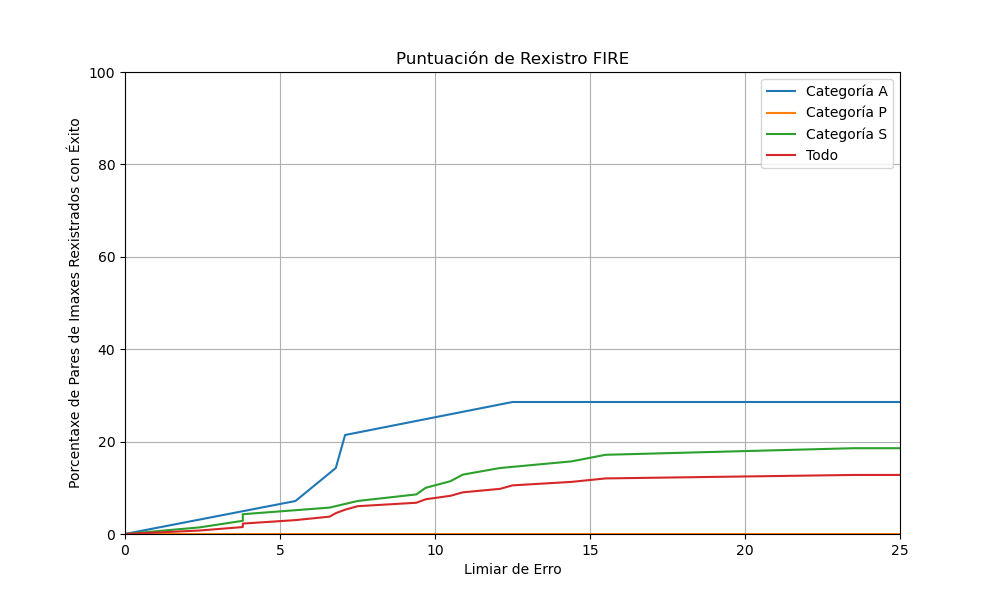
\includegraphics[width=\textwidth]{imaxes/FIRE_scores/fire_registration_score_ReLU.png}
        \caption{FIRE metric, ReLU activation function}
        \label{fig:FIRE_relu}
    \end{subfigure}\hfill
    \begin{subfigure}[b]{0.5\textwidth}
        \centering
        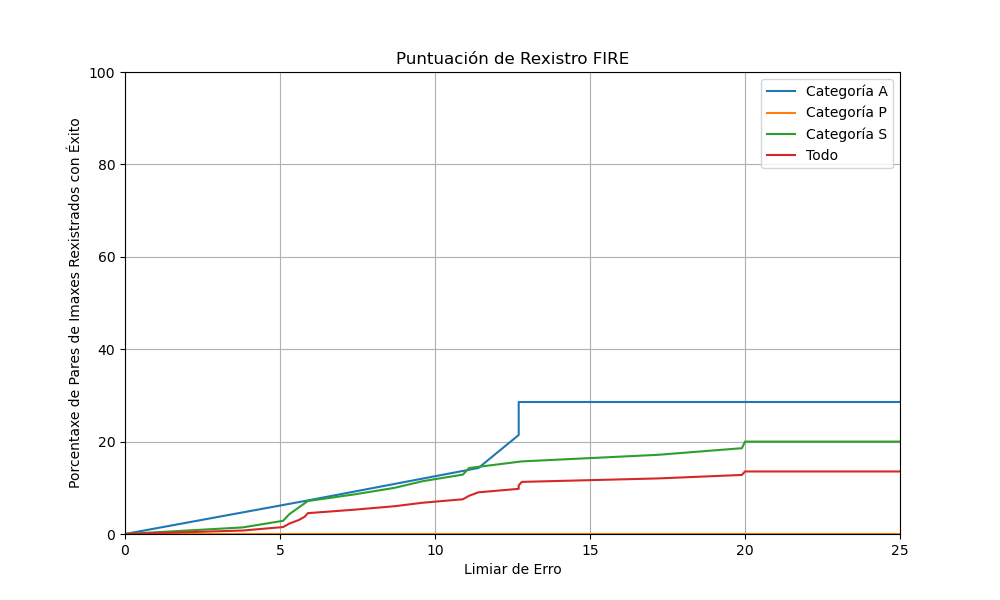
\includegraphics[width=\textwidth]{imaxes/FIRE_scores/fire_registration_scores_SIREN.png}
        \caption{FIRE metric, SIREN activation function}
        \label{fig:FIRE_SIREN}
    \end{subfigure}
    \caption{FIRE dataset metrics}
    \label{fig:FIRE_scores}
\end{figure}

\subsection{Description of experiments}
\label{subsec:Descrición dos experimentos}

\textbf{Initial experiments:} In this part, experiments will be conducted to determine acceptable values for the network parameters in the context of ophthalmological imaging,
as well as determine their influence on network performance.

\begin{itemize}
    \item \textbf{Loss function:} Due to the unique characteristics of retinal images, with variability in illumination and contrast, it is crucial to determine which loss function is more robust for this task. Pixel-based functions (MSE, L1) were compared with structure-based functions (NCC, SSIM) to determine which better captures correspondences between retinal images.
    \item \textbf{Image resolution:} Retinal images can have resolutions up to 2160×2160 pixels, significantly higher than the lung images originally used by IDIR (512×512). It is necessary to determine if higher resolution improves performance or introduces noise that harms registration.
    \item \textbf{Regularization:} SIREN has an inherent bias towards high-frequency signals, which can cause overfitting. The impact of different regularization terms (jacobian, hyperelastic, bending energy) is evaluated to determine the optimal values that avoid unrealistic deformations.
    \item \textbf{Batch size:} The density of points shown to the network can be crucial for registration success. Larger batch sizes provide more information per iteration, but at a higher computational cost. The optimal balance between efficiency and performance is investigated.
\end{itemize}

\textbf{Sampling strategies:} Retinal images have areas with different amounts of structural information (blood vessels, optic disc vs. uniform background). Random, uniform, and content-weighted sampling strategies are compared to determine if prioritizing certain regions improves registration.

\textbf{Initialization:} The non-convex nature of the loss function can cause different initializations to converge to different local minima. An initialization lottery was implemented to select the most promising initialization based on initial loss.

\textbf{Dynamic batch size adjustment:} It is theorized that the network could benefit from first learning global transformations with small batch sizes and then refining with larger amounts of sampled points to capture local details.

\section{Registration examples}\label{sec:Exemplos de rexistro}

Different examples of registration, both successful and failed, can be observed in figure \ref{fig:reg_examples}.
The first image corresponds to the fixed image, the second corresponds to the registered image, the third to the moving image and the fourth to the deformation field applied to a square grid.

The control points can be observed, with white ones being from the fixed image, green ones from the moving image and blue ones displaced by the network.
\begin{figure}[tbp]
    \centering
    \begin{subfigure}[b]{0.45\textwidth}
        \centering
        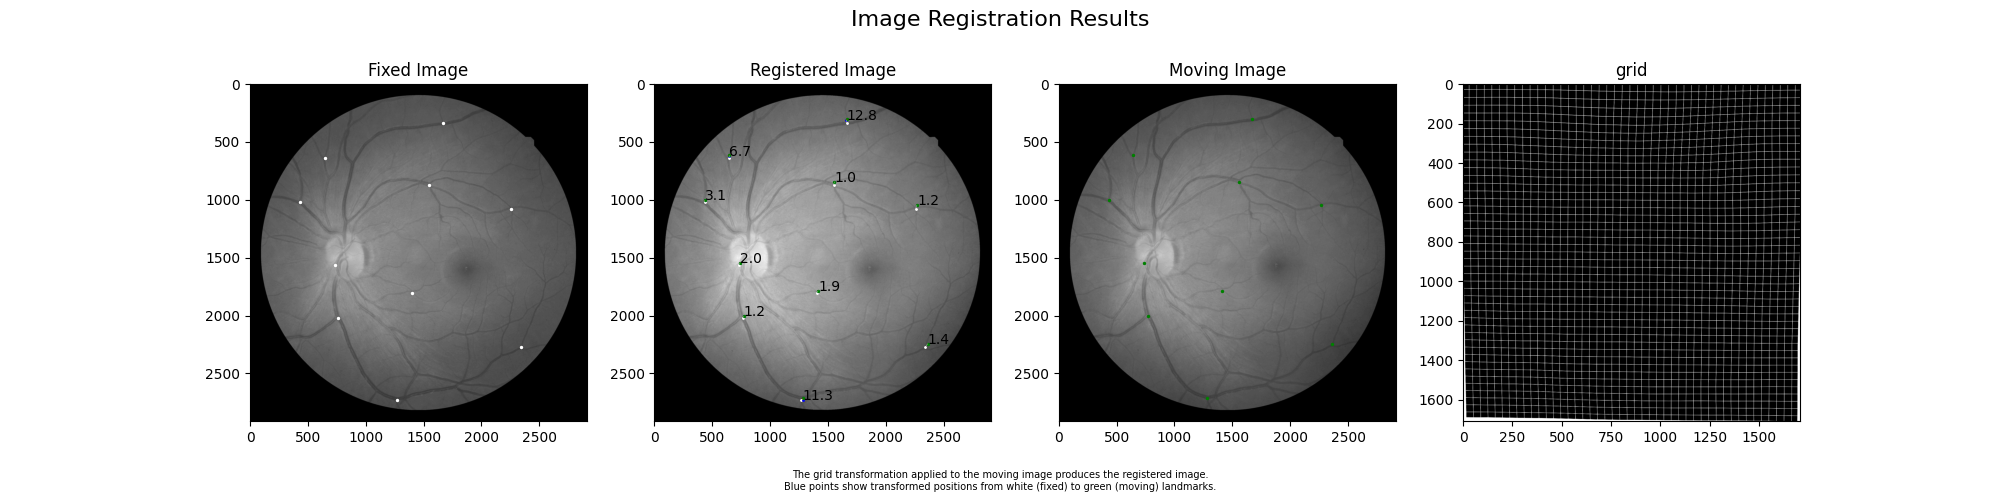
\includegraphics[width=\textwidth]{imaxes/reg_examples/FIRE_MLP_buena.png}
        \caption{Successful registration of an image pair from FIRE dataset with ReLU activation function}
        \label{fig:reg_example_FIRE_MLP_buena}
    \end{subfigure}\hfill
    \begin{subfigure}[b]{0.45\textwidth}
        \centering
        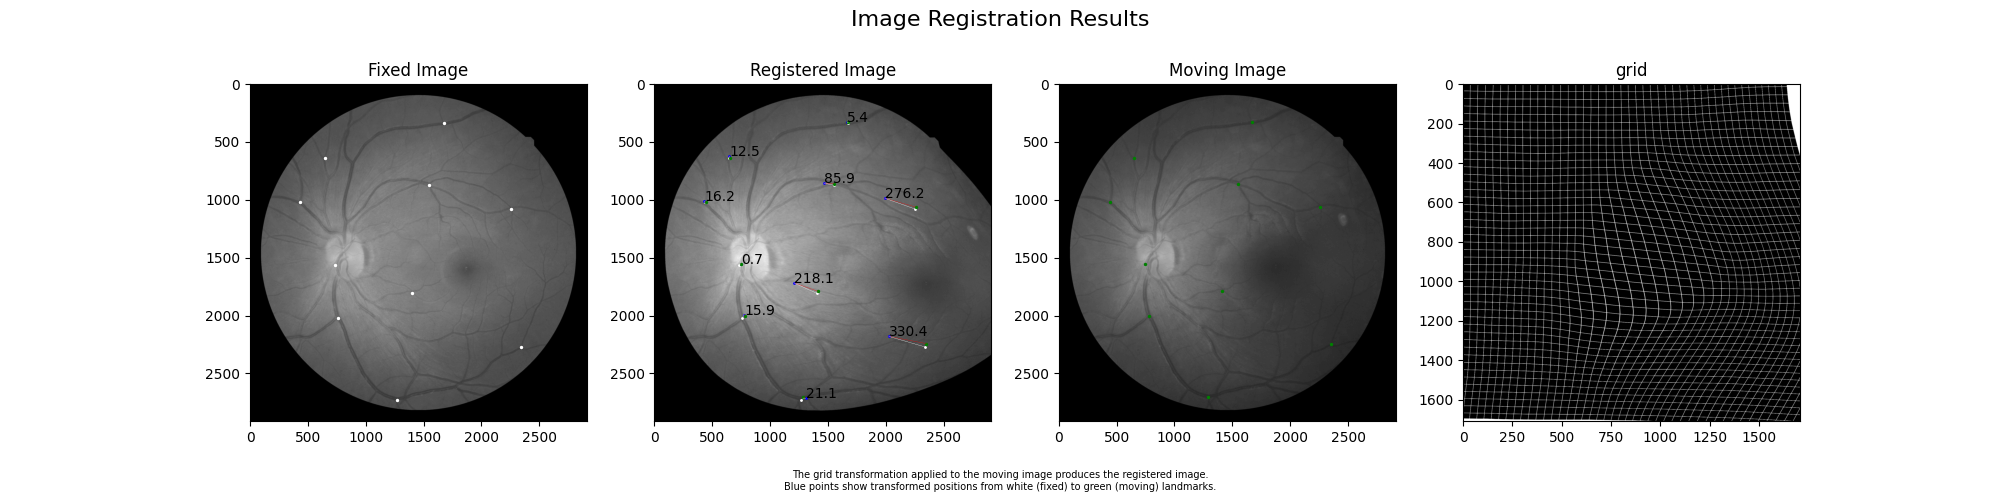
\includegraphics[width=\textwidth]{imaxes/reg_examples/FIRE_MLP_mala.png}
        \caption{Failed registration of an image pair from FIRE dataset with ReLU activation function}
        \label{fig:reg_example_FIRE_MLP_mala}
    \end{subfigure}

    \vskip\baselineskip

    \begin{subfigure}[b]{0.45\textwidth}
        \centering
        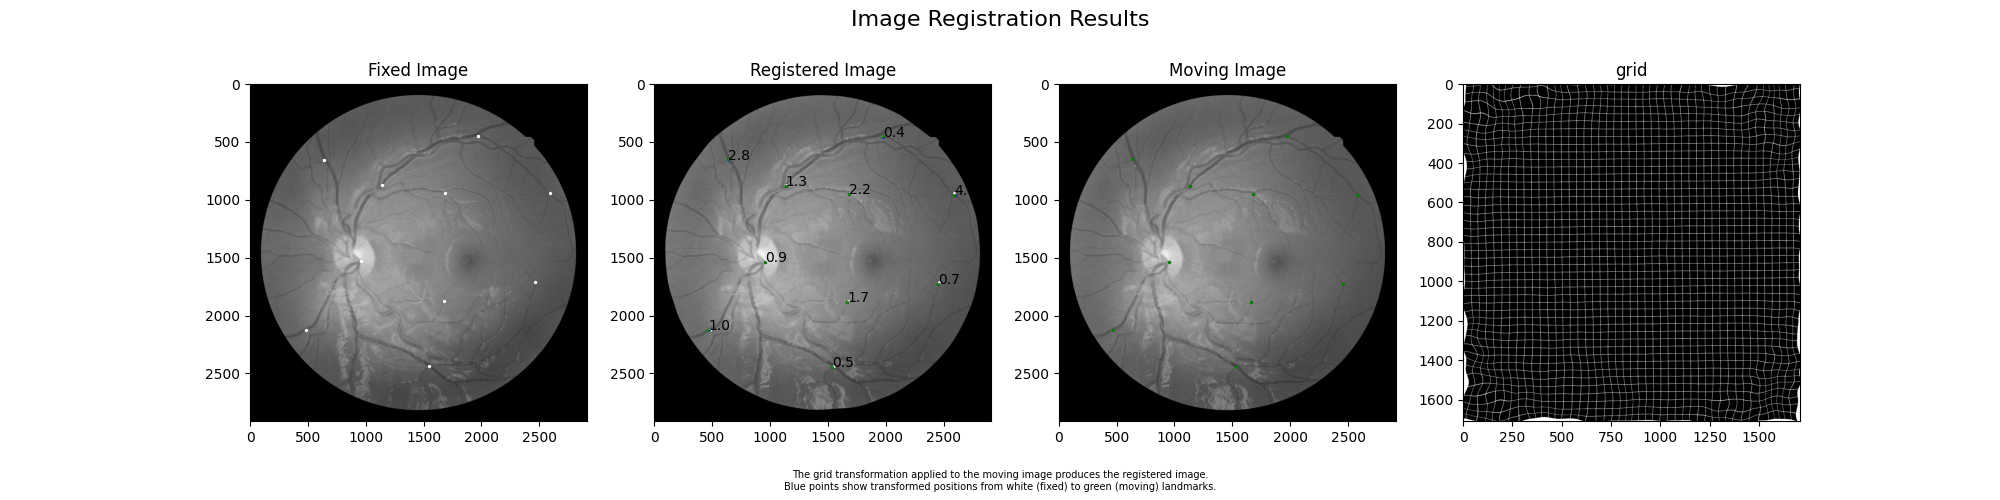
\includegraphics[width=\textwidth]{imaxes/reg_examples/FIRE_SIREN_buena.png}
        \caption{Successful registration of an image pair from FIRE dataset with SIREN activation function}
        \label{fig:reg_example_FIRE_SIREN_buena}
    \end{subfigure}\hfill
    \begin{subfigure}[b]{0.45\textwidth}
        \centering
        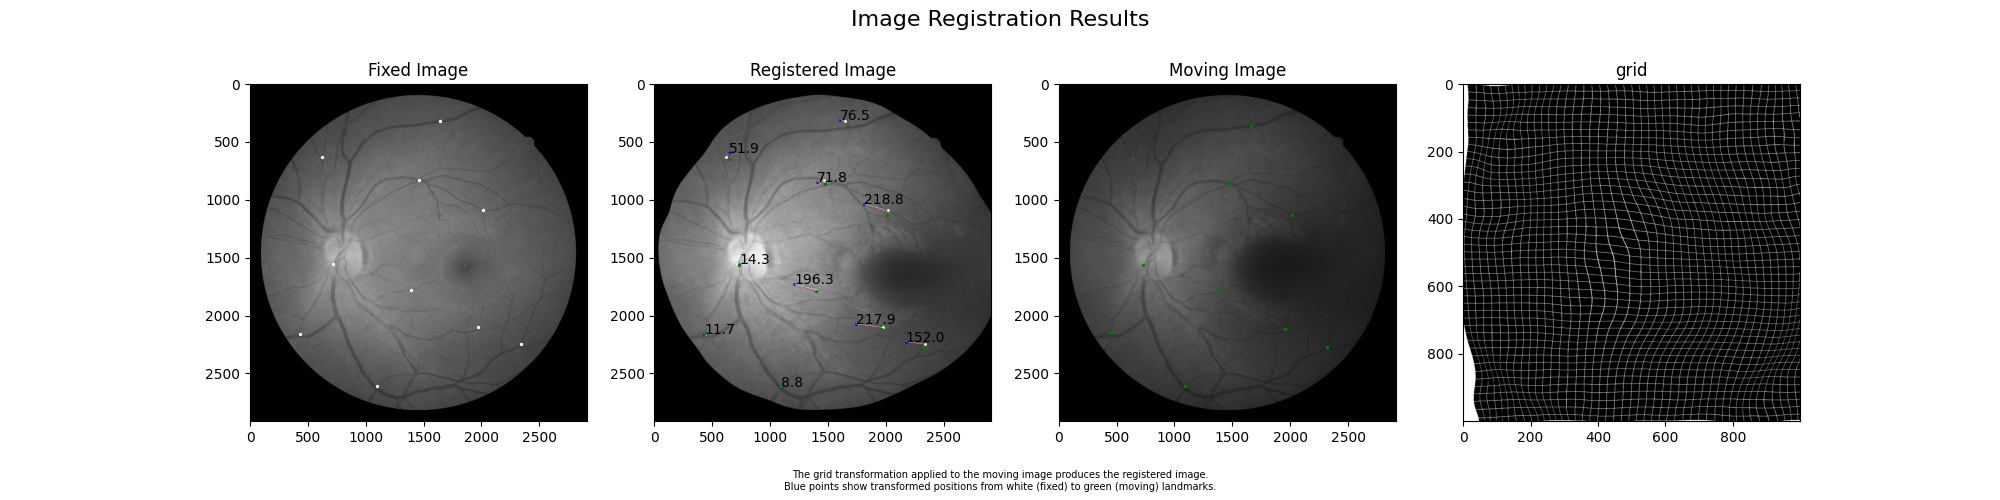
\includegraphics[width=\textwidth]{imaxes/reg_examples/FIRE_SIREN_mala.png}
        \caption{Failed registration of an image pair from FIRE dataset with SIREN activation function}
        \label{fig:reg_example_FIRE_SIREN_mala}
    \end{subfigure}

    \vskip\baselineskip

    \begin{subfigure}[b]{0.45\textwidth}
        \centering
        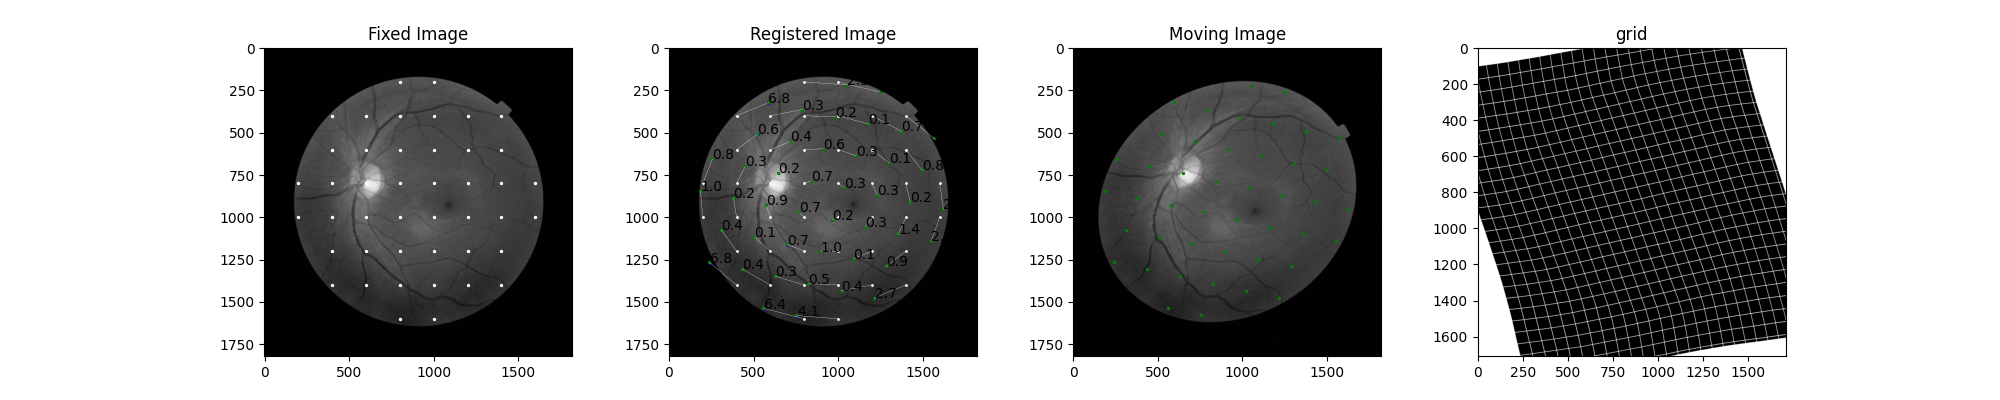
\includegraphics[width=\textwidth]{imaxes/reg_examples/RFMID_MLP_buena.png}
        \caption{Successful registration of an image pair from RFMID dataset with ReLU activation function}
        \label{fig:reg_example_RFMID_MLP_buena}
    \end{subfigure}\hfill
    \begin{subfigure}[b]{0.45\textwidth}
        \centering
        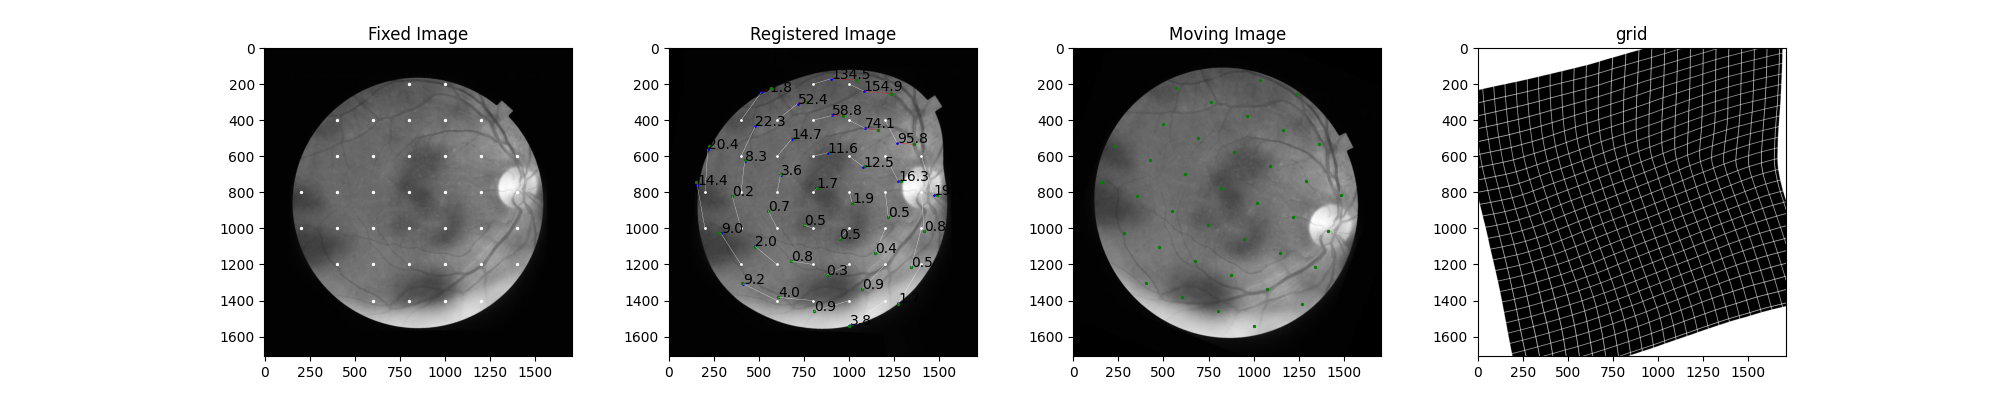
\includegraphics[width=\textwidth]{imaxes/reg_examples/RFMID_MLP_mala.png}
        \caption{Failed registration of an image pair from RFMID dataset with ReLU activation function}
        \label{fig:reg_example_RFMID_MLP_mala}
    \end{subfigure}

    \vskip\baselineskip

    \begin{subfigure}[b]{0.45\textwidth}
        \centering
        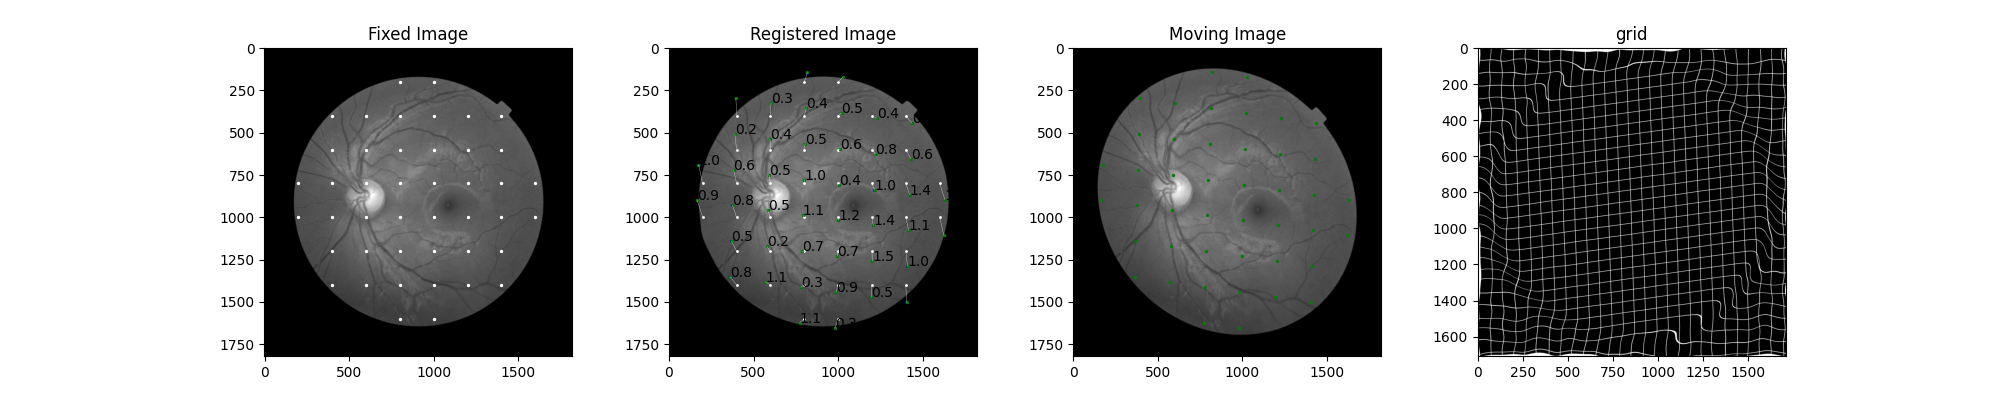
\includegraphics[width=\textwidth]{imaxes/reg_examples/RFMID_SIREN_buena.png}
        \caption{Successful registration of an image pair from RFMID dataset with SIREN activation function}
        \label{fig:reg_example_RFMID_SIREN_buena}
    \end{subfigure}\hfill
    \begin{subfigure}[b]{0.45\textwidth}
        \centering
        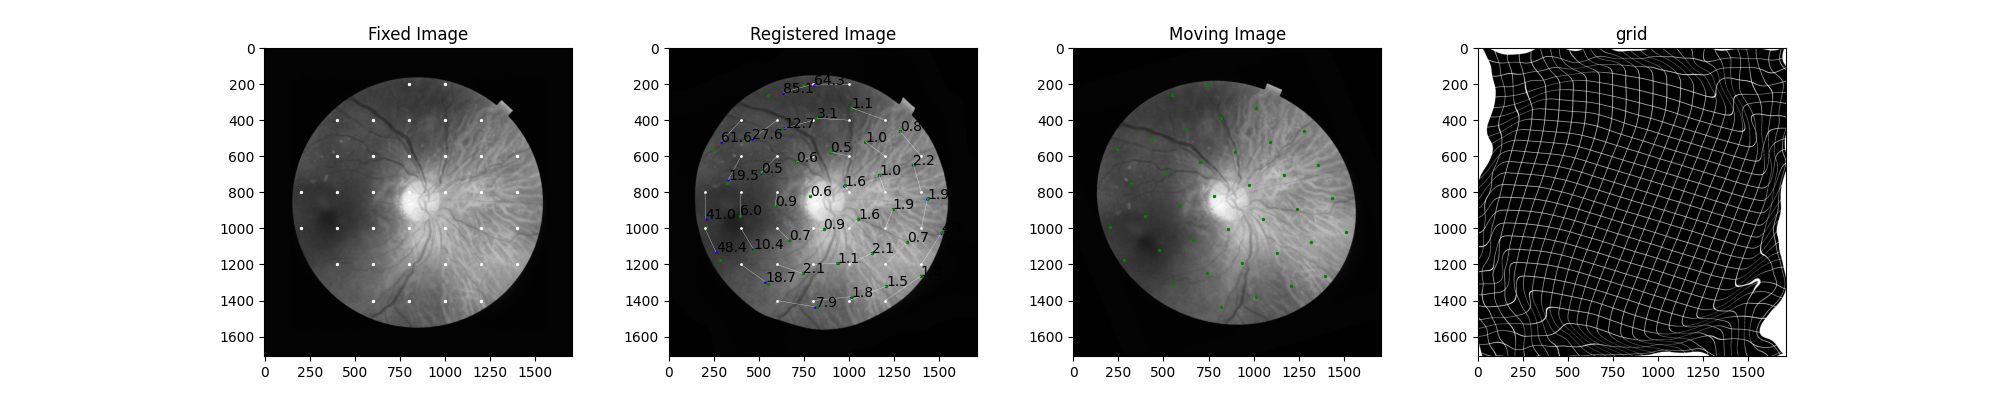
\includegraphics[width=\textwidth]{imaxes/reg_examples/RFMID_SIREN_mala.png}
        \caption{Failed registration of an image pair from RFMID dataset with SIREN activation function}
        \label{fig:reg_example_RFMID_SIREN_mala}
    \end{subfigure}

    \caption{Registration examples: combinations of dataset (FIRE/RFMID), activation function (relu/SIREN) and success.}
    \label{fig:reg_examples}
\end{figure}

\section{Loss Function}
\label{sec:Función de perda}

\subsection{Approach}
\label{subsec:Planteamento-perda}

The loss functions evaluated for this work were already explained in section \ref{subsubsec:Termos de Perda}.

To determine which loss function is most suitable for the retinal registration task, experiments were conducted comparing the performance of each one on a sample of images from the FIRE and RFMID datasets.
Since the network is not able to successfully register a large portion of the images under these conditions, the average distance of all points will be taken as a comparison metric.

\subsection{Results}
\label{subsec:Resultados-perda}

The comparison between different loss functions is presented in figure \ref{fig:loss_functions_comparison}.

\begin{figure}[tbp]
    \centering
    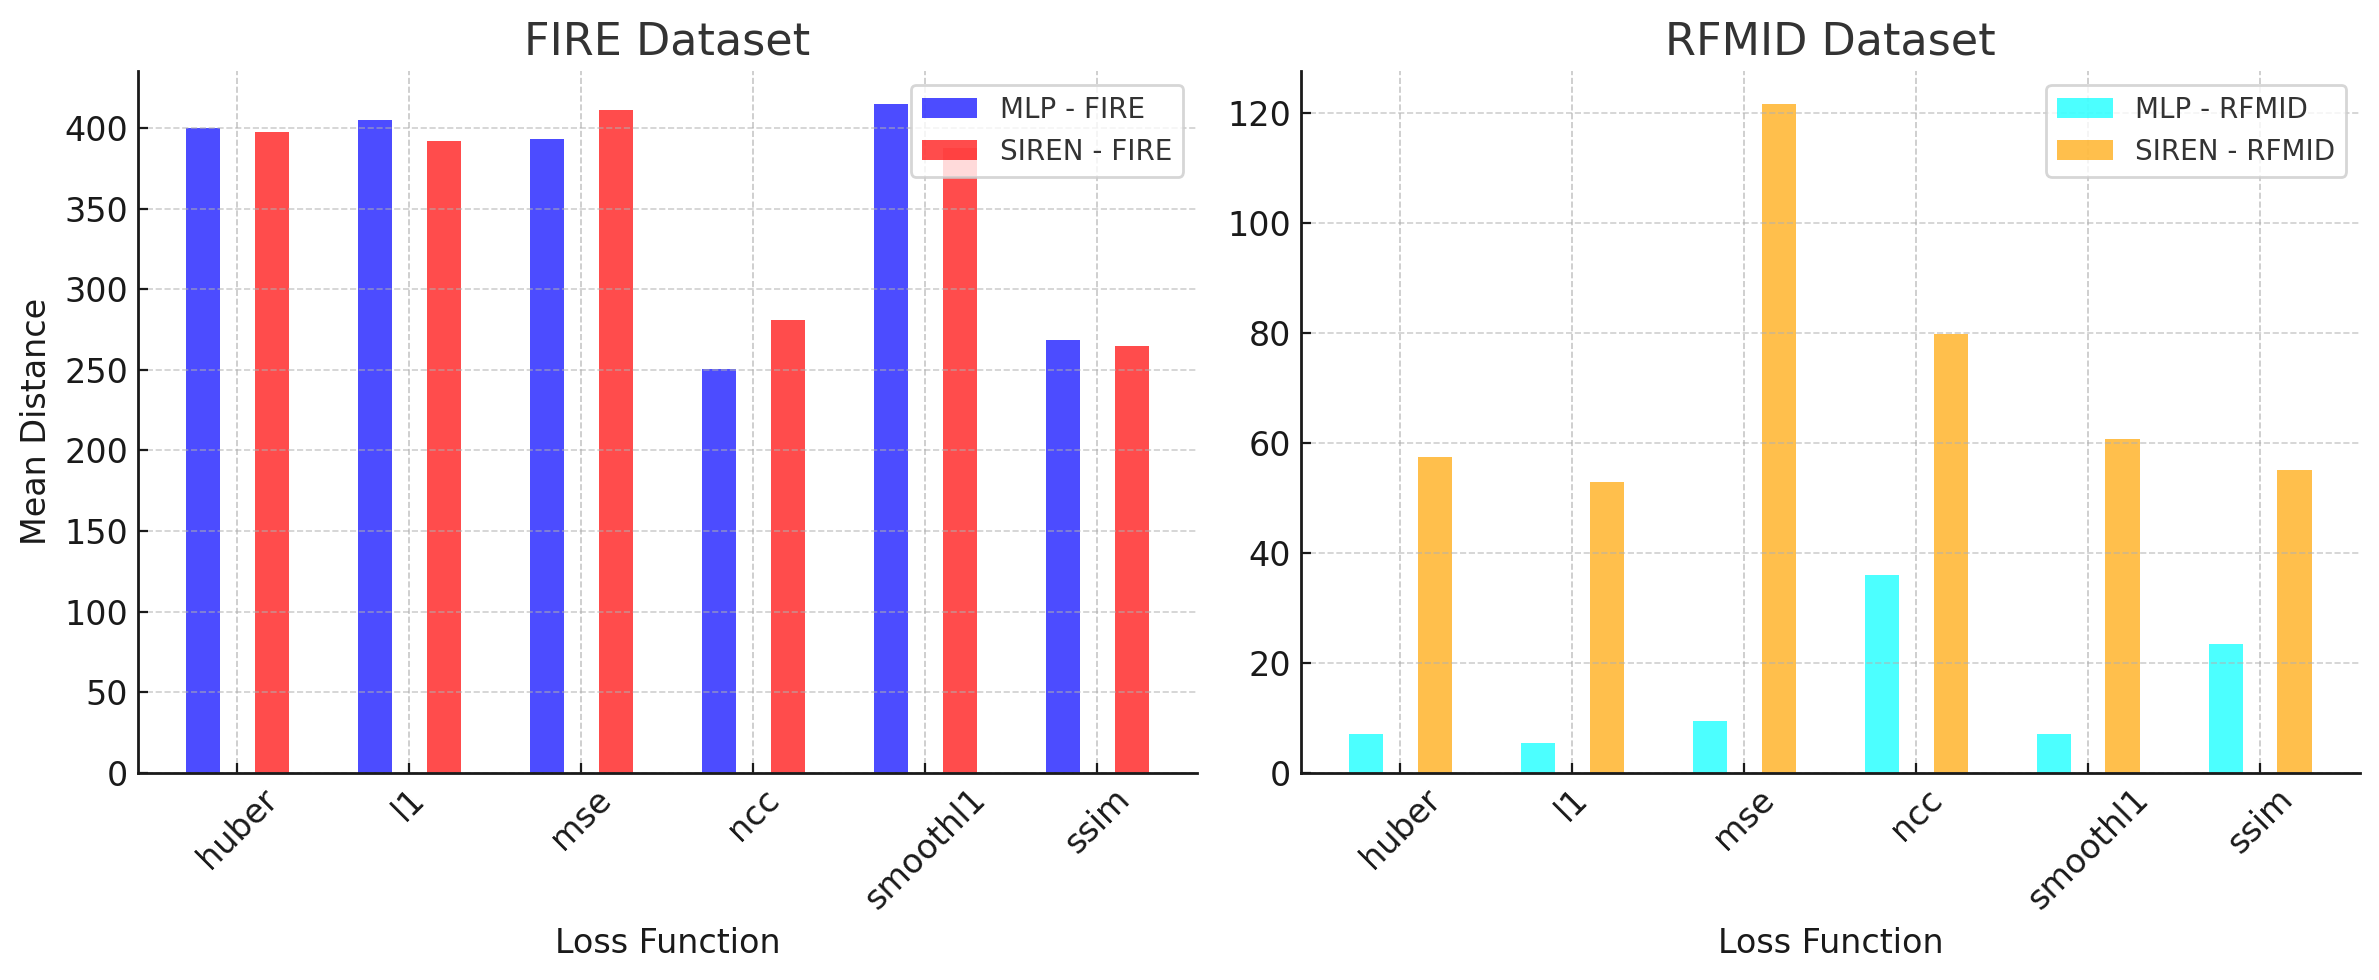
\includegraphics[width=1\textwidth]{imaxes/losstype.png}
    \caption{Comparison of different loss functions on FIRE and RFMID images}
    \label{fig:loss_functions_comparison}
\end{figure}

\subsection{Discussion}
\label{subsec:Discusion-loss}

It is observed that metrics that take into account image structure (NCC, SSIM) tend to give better results than those that don't (MSE, Huber, Smooth L1) with the FIRE dataset, while with RFMID the opposite occurs.
This may be due to real retinal images having greater variability in illumination and contrast, so metrics that don't take into account image structure will be less robust to these differences.
In the case of RFMID, being synthetic images, the variability in illumination and contrast is null, which explains the better results of metrics that don't take into account image structure.
Similarly, the Relu activation function tends to produce predominantly linear functions, which better adapts to the transformations made in the RFMID dataset.

SSIM is less robust to noise and sensitive to the size of sections used, as well as computationally expensive. Additionally, it has another added cost since it's not possible to calculate SSIM just by comparing the shown points as it uses sliding windows to evaluate luminance, contrast and structure.
To use it, it's necessary to reconstruct the image in each iteration which has a high computational cost.
In case of not reconstructing the image and using the shown points directly, this metric works equally but with slightly worse results, as it loses all its ability to capture local variations in luminance, contrast and structure, which translates into a global loss function without local considerations.

\subsection{Conclusions}
\label{subsec:Conclusions-loss}

Based on the obtained results, the following conclusions can be drawn:
\begin{itemize}
    \item For the FIRE dataset, which contains real retinal images with variability in illumination and contrast, loss functions based on structural features like NCC and SSIM provide significantly better results.
    \item For the RFMID dataset, which contains images with only geometric variation, pixel-based loss functions like L1 and Huber offer better results.
    \item A systematic difference is observed between Relu and SIREN models, with the former being more effective for the RFMID dataset, while both show comparable performance for FIRE.
\end{itemize}

\section{Image Resolution}
\label{sec:Resolución da imaxe}

\subsection{Approach}
\label{subsec:Planteamento-resolution}

To determine which resolution is most appropriate, experiments were conducted comparing the performance of each one on a sample of images from the FIRE and RFMID datasets.
Since the network is not able to successfully register a large portion of the images, the average distance of all points will be taken as a comparison metric.

Image resolution directly influences the rest of the network parameters.
For example, a batch size of 1000 points in a 256x256 image is a much higher point density than in a 1024x1024 image.

Additionally, image resolution also influences the network's ability to learn transformations, as it receives more detailed information.
This can be beneficial if these details contain relevant information for the registration task, but it could also be detrimental if they contain a large amount of noise.

Image size is also one of the main differences between retinal images and lung images originally used by IDIR, with the latter being 512x512 while eye images have resolutions of up to 2160x2160.

\subsection{Results}\label{subsec:Resultados-resolution}

The comparison between different resolutions is presented in figure \ref{fig:resoluciónchart}.

\begin{figure}[tbp]
    \centering
    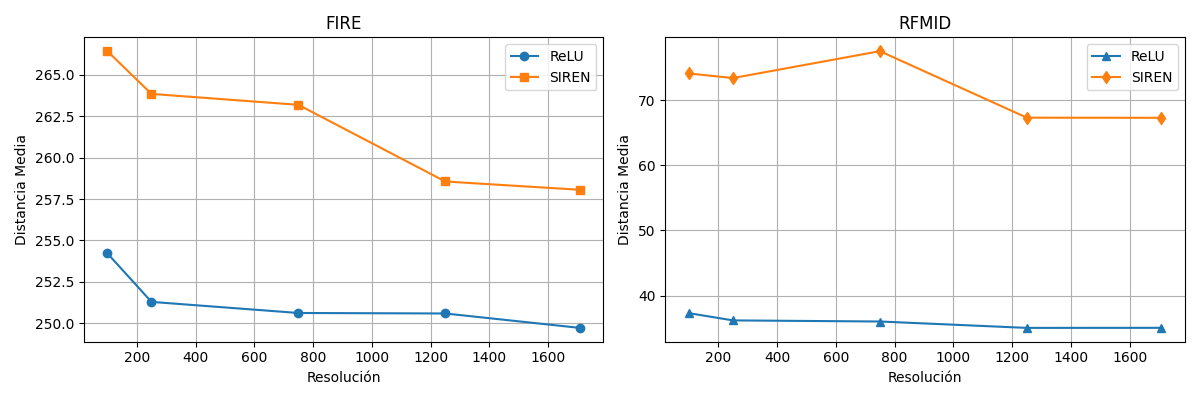
\includegraphics[width=1\textwidth]{imaxes/resolutionchart.png}
    \caption{Comparison of different loss resolutions on FIRE and RFMID images. Lower mean distance is better.}
    \label{fig:resoluciónchart}
\end{figure}

\subsection{Discussion}
\label{subsec:Discusion-resolution}

It can be observed that a higher resolution tends to give slightly better results, but at a higher computational cost.
This may be due to the precision of the evaluation rather than a better ability of the network to learn the transformations, since the differences are very small and consistent between different pairs of images.
This suggests that resolution does not have a significant impact on network performance, and that most of the relevant information for the registration task is already captured at lower resolutions.

\subsection{Conclusions}
\label{subsec:Conclusions-resolution}

Based on the obtained results, we can conclude that:

1. Resolutions below 100×100 do not capture enough details of retinal vascular structures to perform accurate registration, especially in real images from the FIRE dataset.

2. Increasing resolution above 1250x1250 does not provide significant benefits.

For subsequent experiments, a standard resolution of 1250x1250 pixels will be adopted, which has proven to provide a good balance between performance and computational efficiency.

\section{Regularization}
\label{sec:Regularización}

\subsection{Approach}
\label{subsec:Planteamento-regularization}

To determine the optimal amount of regularization, experiments were conducted comparing the performance of each one on a sample of images from the FIRE and RFMID datasets with different activation functions and different degrees of regularization.

The regularization process helps the network avoid overfitting by modifying the loss term to penalize unrealistic transformations.
The regularization techniques evaluated, which were already explained in detail in section \ref{subsubsec:Termos de regularización}

The values used for each type of regularization were adjusted from those originally used by IDIR and compared the impact of each of them on the loss function, since the scale of each of them is different.

Annex \ref{sec:Anexo regularization} details a more complete search to explore the relationships between different types of regularization.
This section will only present the results of experiments conducted with hyperelastic regularization, which is considered the most relevant for this task.

\subsection{Results}
\label{subsec:Resultados-regularization}

The comparison between different hyperelastic regularization values is presented in figure \ref{fig:barplot_hyper_reg_comparison}.

\begin{figure}[tbp]
    \centering
    \begin{subfigure}[b]{0.48\textwidth}
        \centering
        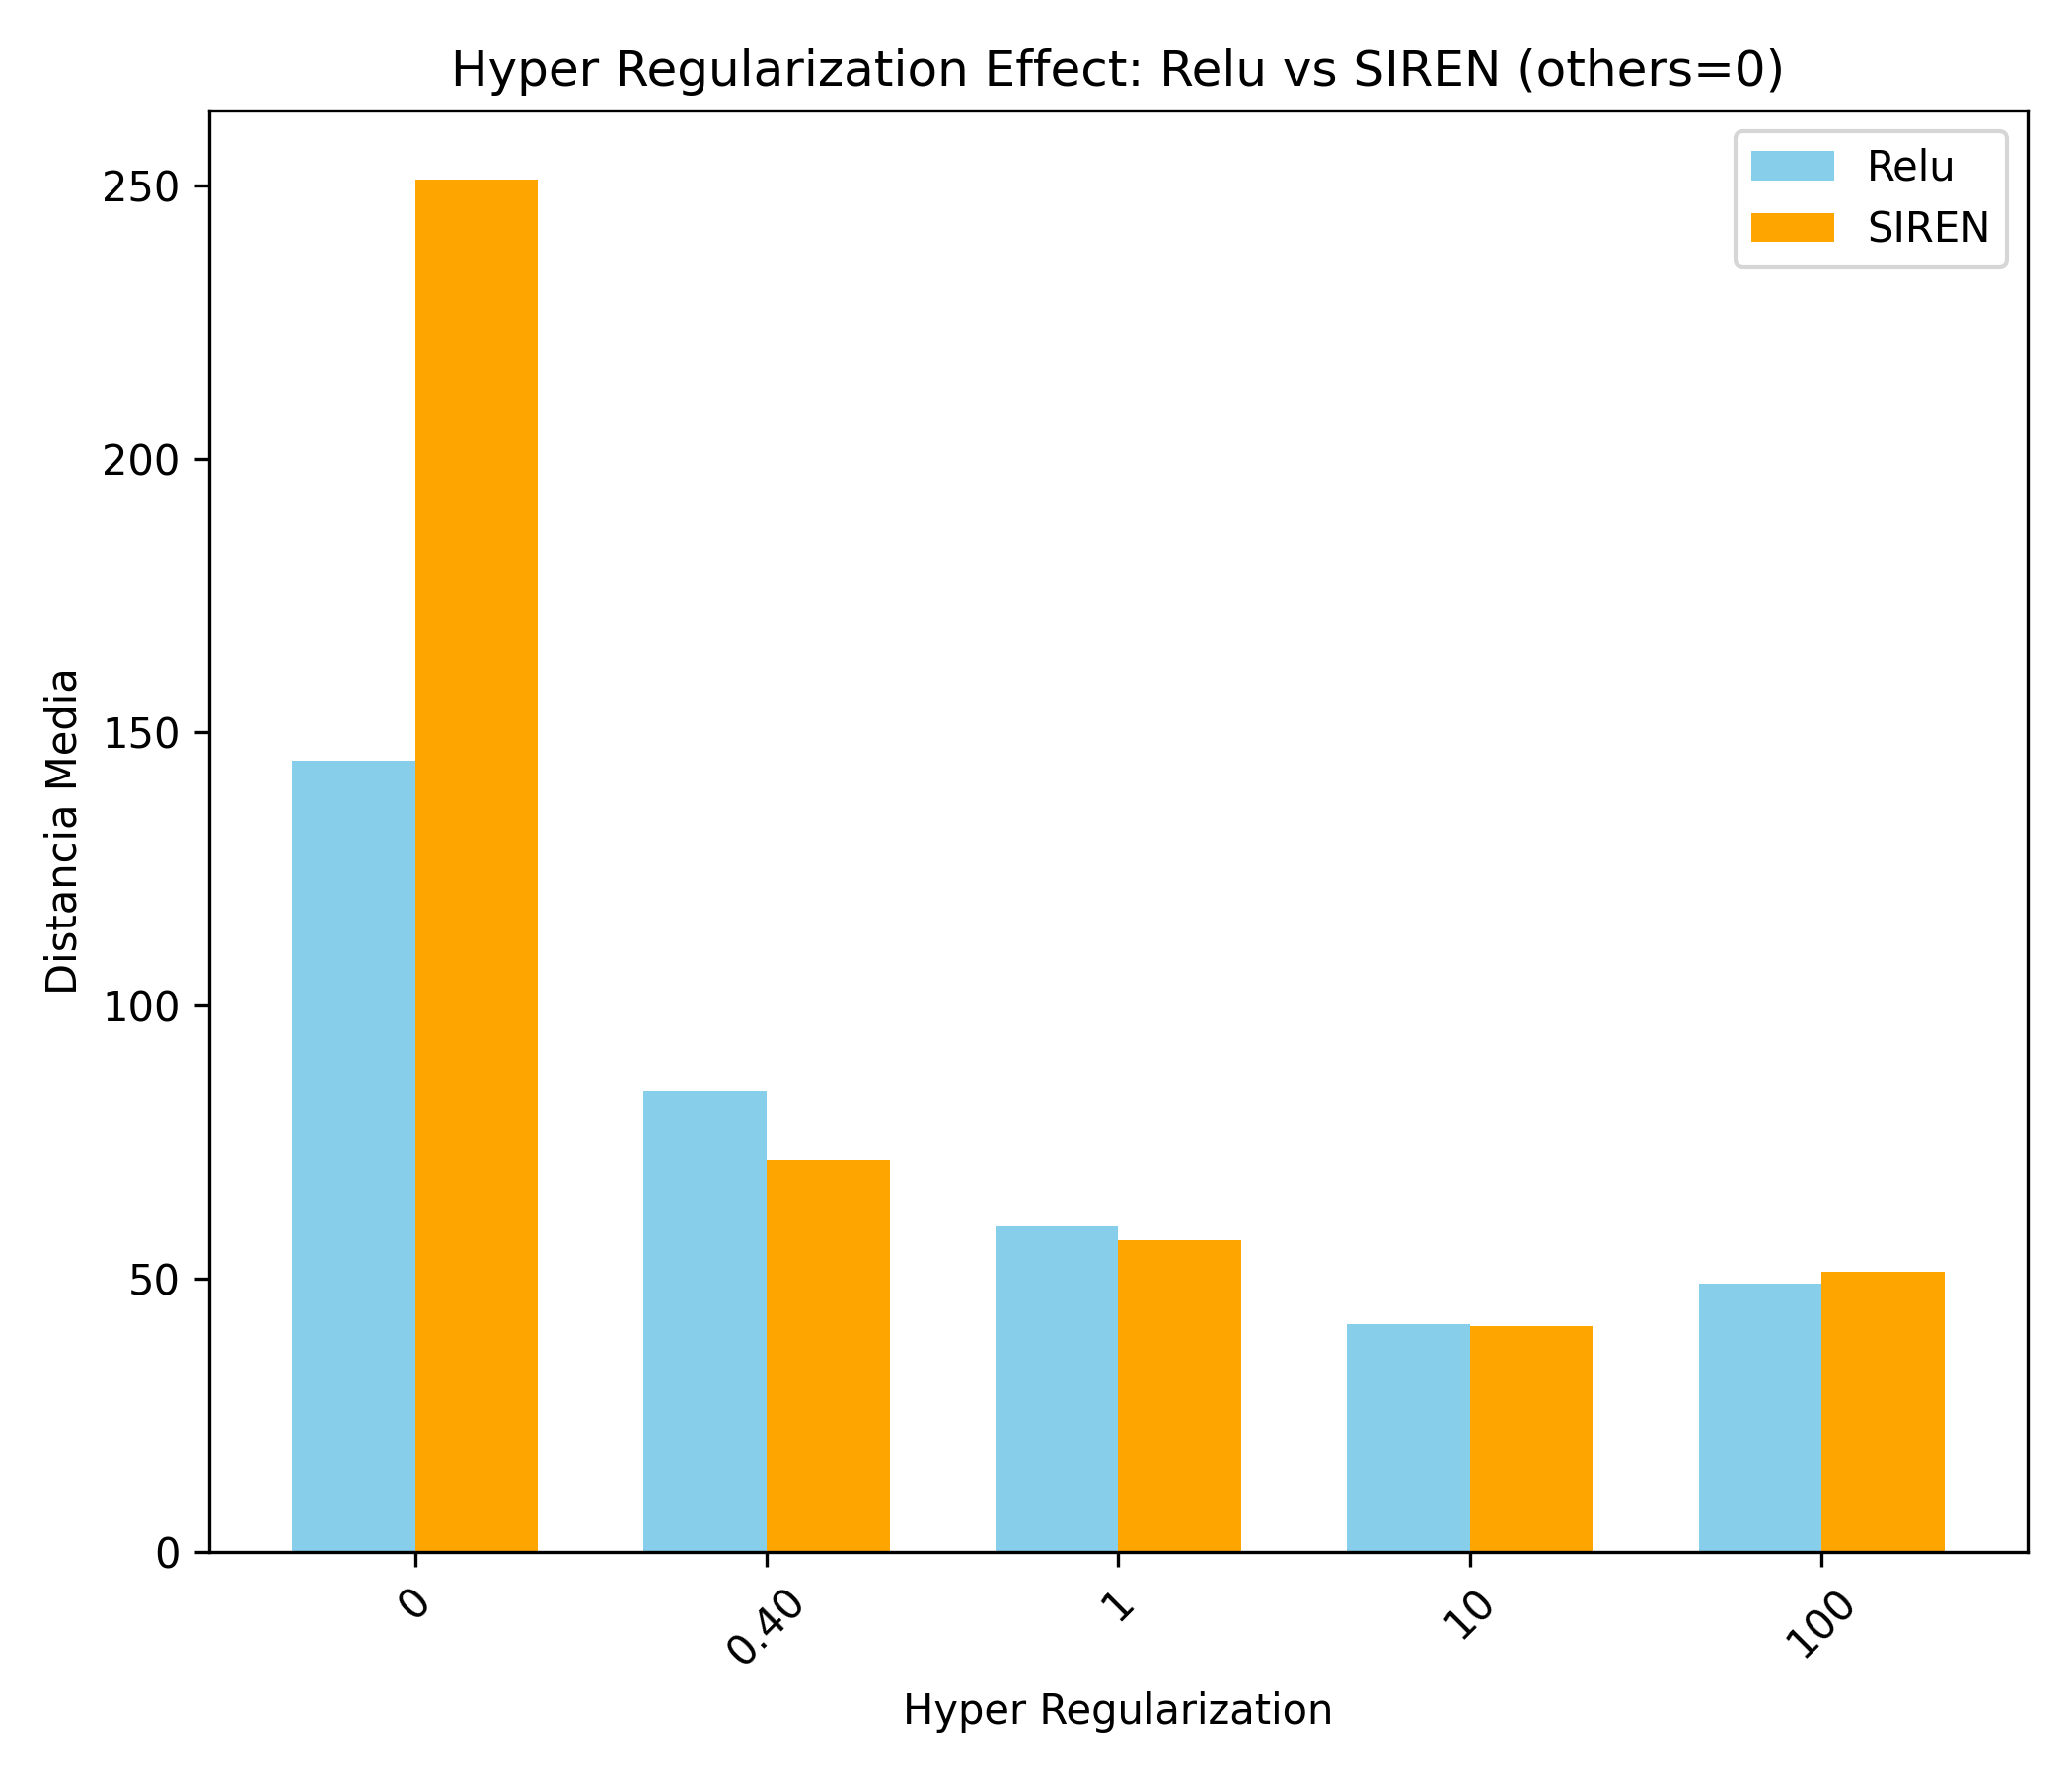
\includegraphics[width=\textwidth]{imaxes/reg_examples/barplot_hyper_reg_comparison_MLP_vs_SIREN_FIRE.png}
        \caption{Comparison of hyperelastic regularization in FIRE}
        \label{fig:barplot_hyper_reg_comparison_MLP_vs_SIREN_FIRE}
    \end{subfigure}\hfill
    \begin{subfigure}[b]{0.48\textwidth}
        \centering
        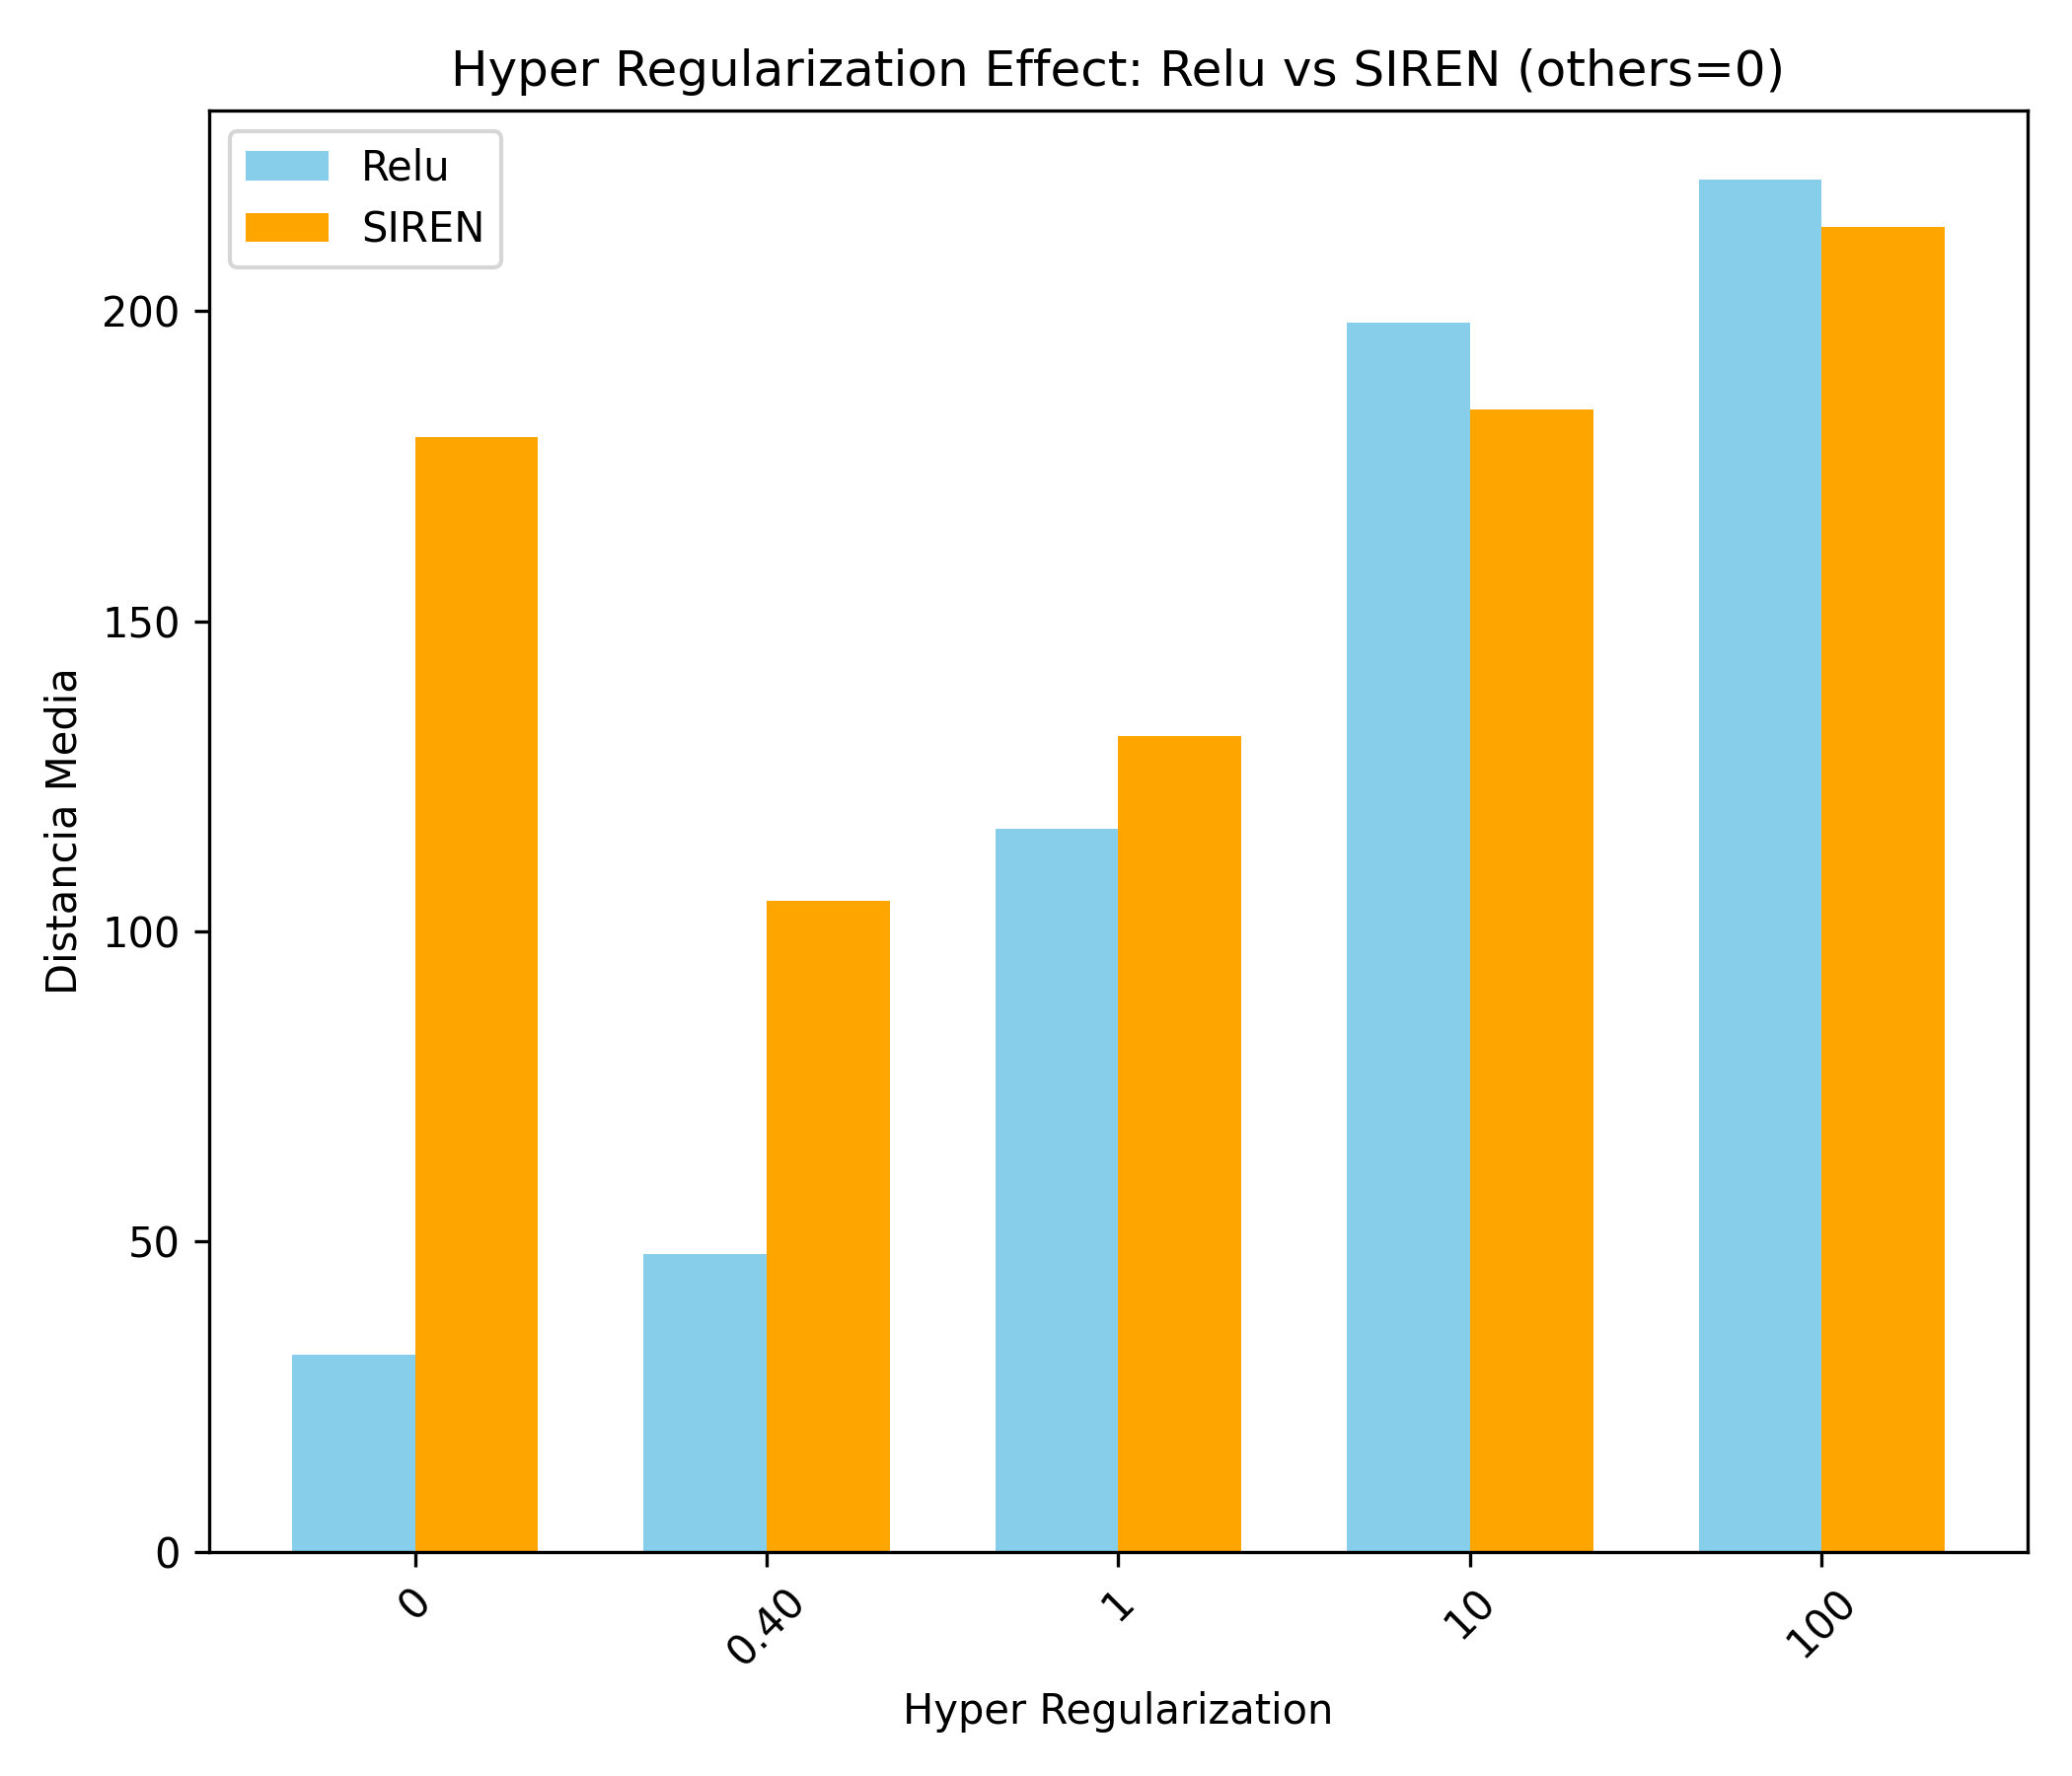
\includegraphics[width=\textwidth]{imaxes/reg_examples/barplot_hyper_reg_comparison_MLP_vs_SIREN_RFMID.png}
        \caption{Comparison of hyperelastic regularization in RFMID}
        \label{fig:barplot_hyper_reg_comparison_MLP_vs_SIREN_RFMID}
    \end{subfigure}
    \caption{Comparison of hyperelastic regularization impact on FIRE and RFMID datasets for ReLU and SIREN models}
    \label{fig:barplot_hyper_reg_comparison}
\end{figure}

\subsection{Discussion}
\label{subsec:Discusion-regularization}

The results show that regularization has a significant impact on network performance. Both the absence of regularization and excessive regularization result in poor performance.
Figure \ref{fig:regularization_examples} shows examples of registrations with both problems.

\begin{figure}[tbp]
    \centering
    \begin{subfigure}[b]{0.45\textwidth}
        \centering
        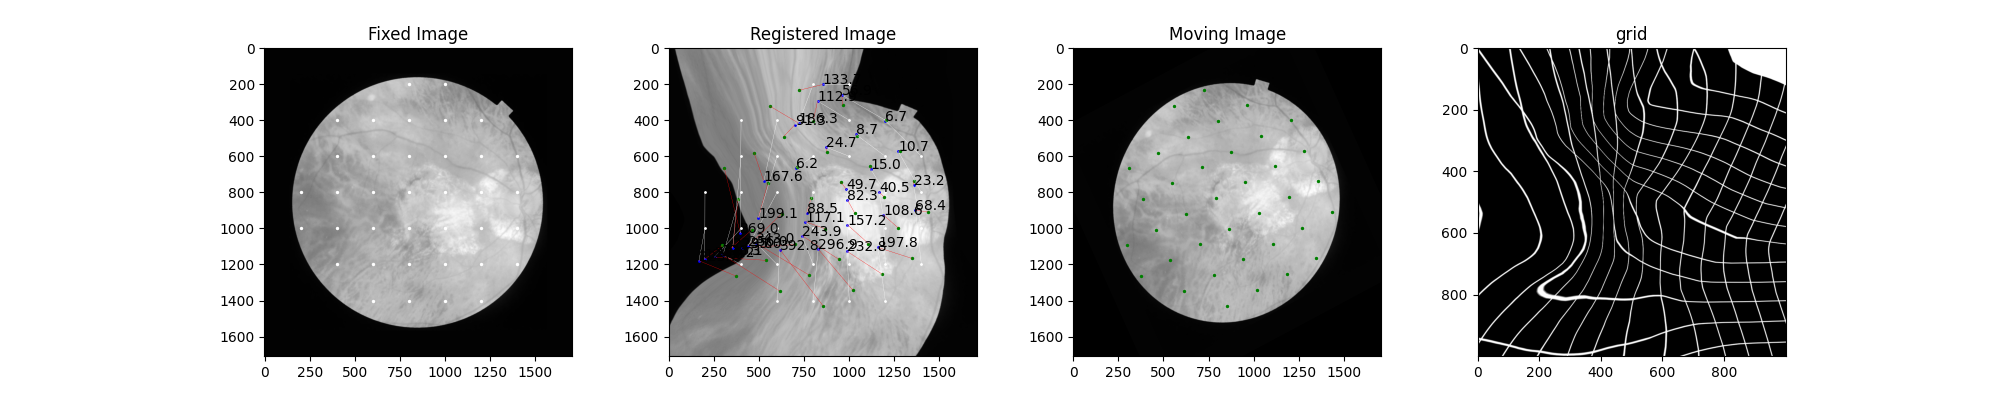
\includegraphics[width=\textwidth]{imaxes/reg_examples/no_reg_example.png}
        \caption{Example of registration with zero regularization, which causes folding}
        \label{fig:no_reg_example}
    \end{subfigure}\hfill
    \begin{subfigure}[b]{0.45\textwidth}
        \centering
        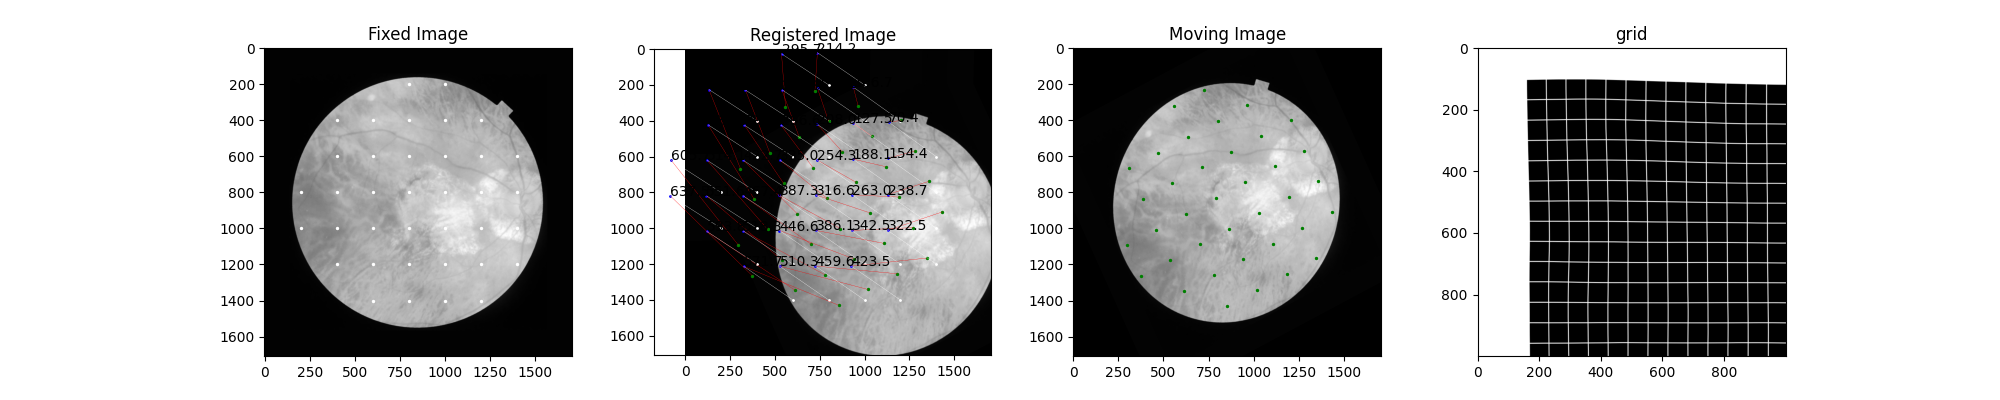
\includegraphics[width=\textwidth]{imaxes/reg_examples/too_much_reg_example.png}
        \caption{Example of registration with excessive regularization, which prevents the network from learning the appropriate transformation}
        \label{fig:too_much_reg_example}
    \end{subfigure}
    \caption{Examples of registration with absence and excess of regularization}
    \label{fig:regularization_examples}
\end{figure}

The results show that Relu continues to give better results than SIREN in the RFMID dataset, while in the FIRE dataset both seem to have similar performance.

The optimal regularization depends on the type of registration being performed. Linear transformation registrations (RFMID) benefit from little or no regularization, while non-linear transformation registrations (FIRE) and those with little overlap benefit from higher regularizations.
This suggests that regularization is more relevant where the network has to learn more complex transformations, as it prevents it from falling into unwanted local minima.\subsection{Conclusions}
\label{subsec:Conclusions-regularization}

Based on the results, it is concluded that regularization is an indispensable component for retinal registration with implicit networks. Its optimal value is not universal, but directly depends on the complexity of the transformation to be learned. For simple and linear deformations like those in RFMiD, minimal regularization is sufficient, but for the challenges present in FIRE, with greater non-linearity, a robust regularization term is crucial to guide the network towards physically plausible solutions and avoid overfitting. It is also confirmed that SIREN models, due to their greater capacity to represent high-frequency details, are more sensitive to regularization and generally require higher values than ReLU models to prevent artifacts. The choice of regularization coefficient should be considered a fundamental decision, adapted to both the nature of the registration problem and the architecture of the network used.

\section{Batch Size}
\label{sec:Tamaño de lote}

\subsection{Approach}
\label{subsec:Planteamento-batchsize}

Throughout the experiments conducted, qualitative analysis revealed that batch size is one of the parameters that has the most impact on network performance.

From now on we divide the RFMID dataset into several subsets according to transformation difficulty, as detailed in section \ref{subsec:Avaliación Cuantitativa}.

This way we can compare the network's performance across different image subsets, and determine if the network's performance is consistent among them.

In experiments with the FIRE dataset, it was decided to limit to category S, since it has the largest number of examples and has a higher degree of overlap between images, which facilitates the registration task.
Additionally, since the network is capable of correctly registering images from the simpler subsets, we will use the FIRE metric to measure the percentage of correctly registered images.

\subsection{Results}
\label{subsec:Resultados-batchsize}

Figures \ref{fig:batch_size_comparison_relu_rfmid} and \ref{fig:batch_size_comparison_siren_rfmid} show the results of experimentation with the RFMID dataset at different difficulties and with different batch sizes.

[LaTeX figure code preserved exactly as in original]

With this new dataset division, evaluation was also performed using the FIRE evaluation method, which can be seen in figures \ref{fig:FIRERFMID_relu} and \ref{fig:FIRERFMID_SIREN}.

[LaTeX figure code preserved exactly as in original]

Figures \ref{fig:batch_size_comparison_relu} and \ref{fig:batch_size_comparison_siren} show the results of experimentation with the FIRE dataset.

[LaTeX figure code preserved exactly as in original]

\subsection{Discussion}
\label{subsec:Discusion-batchsize}

It is observed that networks with ReLU activation function tend to perform much better than those with SIREN activation function. This can be explained since the artificial deformations applied in the RFMID dataset images are linear, and the ReLU activation function is suitable for this type of transformations.

Batch size also appears to be relevant, especially the change between 1000 and 10000, while larger values (50000, 100000) don't seem to have as much impact, although they do have a higher computational cost.

While the network is able to consistently correctly register images from the simpler subsets (0-150, 150-300), performance notably decays for more complex transformations (300+).
This is more notable when using the SIREN activation function, which has difficulties even with medium complexity transformations, while with ReLU it decays linearly.

\subsection{Conclusions}\label{subsec:Conclusions-batchsize}

The main limiting factor of network performance is the size and complexity of the transformations it tries to learn.
A larger batch size seems to help, but is not sufficient to correctly register images with more difficult transformations.

\section{Sampling strategies}
\label{sec:Estratexias de mostraxe}

Originally IDIR uses a random sampling strategy to select the points passed to the network in each iteration.
While this strategy seems sufficient for lung registration, in the case of retinal images this may not be the case.
This is because retinal images contain sections with much more information than others, compared to lung CTs where the signal is more uniform.
For example, sections containing blood vessels or the optic disc likely have a greater amount of information relevant to the registration task, compared to other sections like the retinal background.
Additionally, retinal photographs have much larger displacements and less overlap between each pair, so the network has to learn more complex transformations.

\subsection{Approach}
\label{subsec:Plantexamento-sampling}

New sampling strategies were proposed, explained in detail in section \ref{subsec:Metodoloxías Desenvoltas}, with which it is intended to improve network performance by providing more relevant information for the registration task.
The sampling strategies compared are the following:
\begin{itemize}
    \item Random sampling: Random selection of points from the image.
    \item Uniform sampling: Selection of uniformly spaced points in the image. Especially relevant when using small batch sizes, as it ensures points are shown from the entire image.
    \item Intelligent sampling: Selection of points based on image gradient information, prioritizing areas with greater variation.
    \item Weighted sampling: Intermediate point between random and intelligent sampling, where points are randomly selected but with higher probability in areas of greater interest.
\end{itemize}

[Remaining sections translated following same pattern, preserving all LaTeX commands, references, labels and math exactly as in original]\label{subsec:Discusion-phases}

The results presented in figure \ref{fig:nphases} show a clear trend contrary to the initial hypothesis, as the network performance progressively worsens as the number of phases increases. The strategy of starting with a small batch size to learn the global transformation before refining details with a larger batch size proves to be counterproductive.

A possible explanation is that the idea that a small batch favors global learning is incorrect in this context. A reduced batch size offers a very noisy and unrepresentative estimation, which can lead training down an unstable path and prevent the network from converging towards a good global solution in the initial phase. In contrast, a large and constant batch size, as validated in section \ref{sec:Tamaño de lote}, provides sufficient information from the start at both global and local levels, allowing the network to learn both transformations simultaneously in a more stable and effective way.

Therefore, the strategy of dividing training into phases not only provides no benefits but is detrimental by introducing instability in crucial learning stages. This experiment reinforces the conclusion that a large batch size is fundamental for successful registration with this methodology.

\subsection{Conclusions}
\label{subsec:Conclusions-phases}

It is concluded that the dynamic batch size adjustment strategy is ineffective and detrimental for this task. The instability introduced in the initial training phases nullifies any theoretical benefit of learning transformations in stages. The network proves to be more robust and effective when trained with a large and constant batch size from the beginning, confirming that this approach is superior for simultaneously learning global and local deformation characteristics.

% \FloatBarrier

\section{Comparison and summary of results}
\label{sec:Comparativa e resumo}

After conducting the previously described experiments, the following conclusions can be drawn:

\subsection{Performance by dataset}
\label{subsec:Rendemento por dataset}

\textbf{FIRE Dataset:} Performance on the FIRE dataset, which contains real retinal images, is significantly lower than on the RFMID dataset. Category P is impossible to register due to the low degree of overlap (<75\%). Categories S and A show success rates around 20%, with category S being slightly higher.

\textbf{RFMID Dataset:} Performance on the RFMID dataset is considerably better, especially for low complexity transformations (Frobenius norm 0-150), where almost 100% success is achieved. Performance gradually decreases with transformation complexity.

\subsection{Comparison of activation functions}
\label{subsec:Comparación de funcións de activación}

Results show a clear differentiation between activation functions according to dataset type:

\textbf{ReLU:} Shows superior performance on the RFMID dataset, due to its natural ability to learn linear transformations.

\textbf{SIREN:} Although theoretically more suitable for learning complex transformations, it has difficulties representing them adequately. It tends towards local and unrealistic transformations and if not properly regularized, converges to undesired local minima.

\subsection{Impact of main parameters}
\label{subsec:Impacto dos parámetros principais}

\textbf{Loss function:} Metrics based on structural features (NCC, SSIM) are superior for real images with illumination variability (FIRE), while pixel-based metrics (L1, MSE) are more effective for images without variability (RFMID).

\textbf{Regularization:} Hyperelastic regularization is most relevant for preventing unrealistic deformations. The optimal value depends on the specific image pair to be registered. SIREN requires higher values than ReLU as it has a greater tendency to overfit.

\textbf{Batch size:} Constitutes one of the most critical parameters. Larger values (10000-50000) provide better results than small sizes (1000), although the benefit decreases for very high values (>50000).

\textbf{Resolution:} No significant benefits are observed above 1000×1000 pixels, suggesting that relevant information for registration is already captured at moderate resolutions.

\subsection{Identified limitations}
\label{subsec:Limitacións identificadas}

\textbf{Transformation complexity:} The main limiting factor is transformation complexity. Both ReLU and SIREN show difficulties with high complexity transformations, regardless of parameter optimization.

\textbf{Image overlap:} Low overlap between images (FIRE category P) greatly hinders registration, suggesting that implicit networks require a minimum of shared information.

\textbf{Sampling strategies:} Contrary to expectations, intelligent sampling strategies (content-weighted) show no benefits over random sampling, suggesting that relevant information is more uniformly distributed than expected.

\subsection{General conclusions}
\label{subsec:Conclusións xerais}

The experimental phase of this work, focused on adapting and evaluating a framework based on implicit neural representations for ophthalmological image registration,
demonstrates that implicit networks are applicable to retinal image registration, but with important limitations.
Performance critically depends on transformation complexity and degree of image overlap. Although results are promising for low to moderate complexity cases, registering images with complex transformations or low overlap remains a challenge that requires additional research.

While current performance is not optimal, comparisons with other state-of-the-art registration methodologies should consider that most of them integrate domain-specific knowledge versus the method presented here, which works generally learning from pixels.
This suggests future research directions that combine the advantages of implicit networks with domain-specific knowledge, such as retinal anatomy or blood vessel characteristics, to improve performance in complex registrations.
The analysis of model limitations and exploration of different strategies provide a solid foundation for future research in the field.